% https://johncarlosbaez.wordpress.com/2021/12/08/the-madelung-rules/
\documentclass[tikz,border=4pt]{standalone}
\usetikzlibrary{matrix,arrows.meta,calc,backgrounds}
\def\tg{\fpeval{atand(\deltay/\deltax)}}
\def\angleA{\fpeval{90+\tg}}
\def\angleB{\fpeval{\angleA+180}}
\def\angleC{\fpeval{\angleA-180}}
\def\mynodesize{.6}
\def\colsep{2}
\def\rowsep{1}
\def\myR{\fpeval{cosd(\tg)*(\rowsep+\mynodesize)*0.25}}
\def\deltax{1.2}
\def\deltay{.6}
\tikzset{
  orb/.style={
    circle,draw=black,thick,
    inner sep=0pt,minimum size=\mynodesize cm,
    font=\sffamily\bfseries\small
},
  s/.style={orb,fill=yellow},
  p/.style={orb,fill=green},
  d/.style={orb,fill=cyan},
  f/.style={orb,fill=lime}
}
\begin{document}


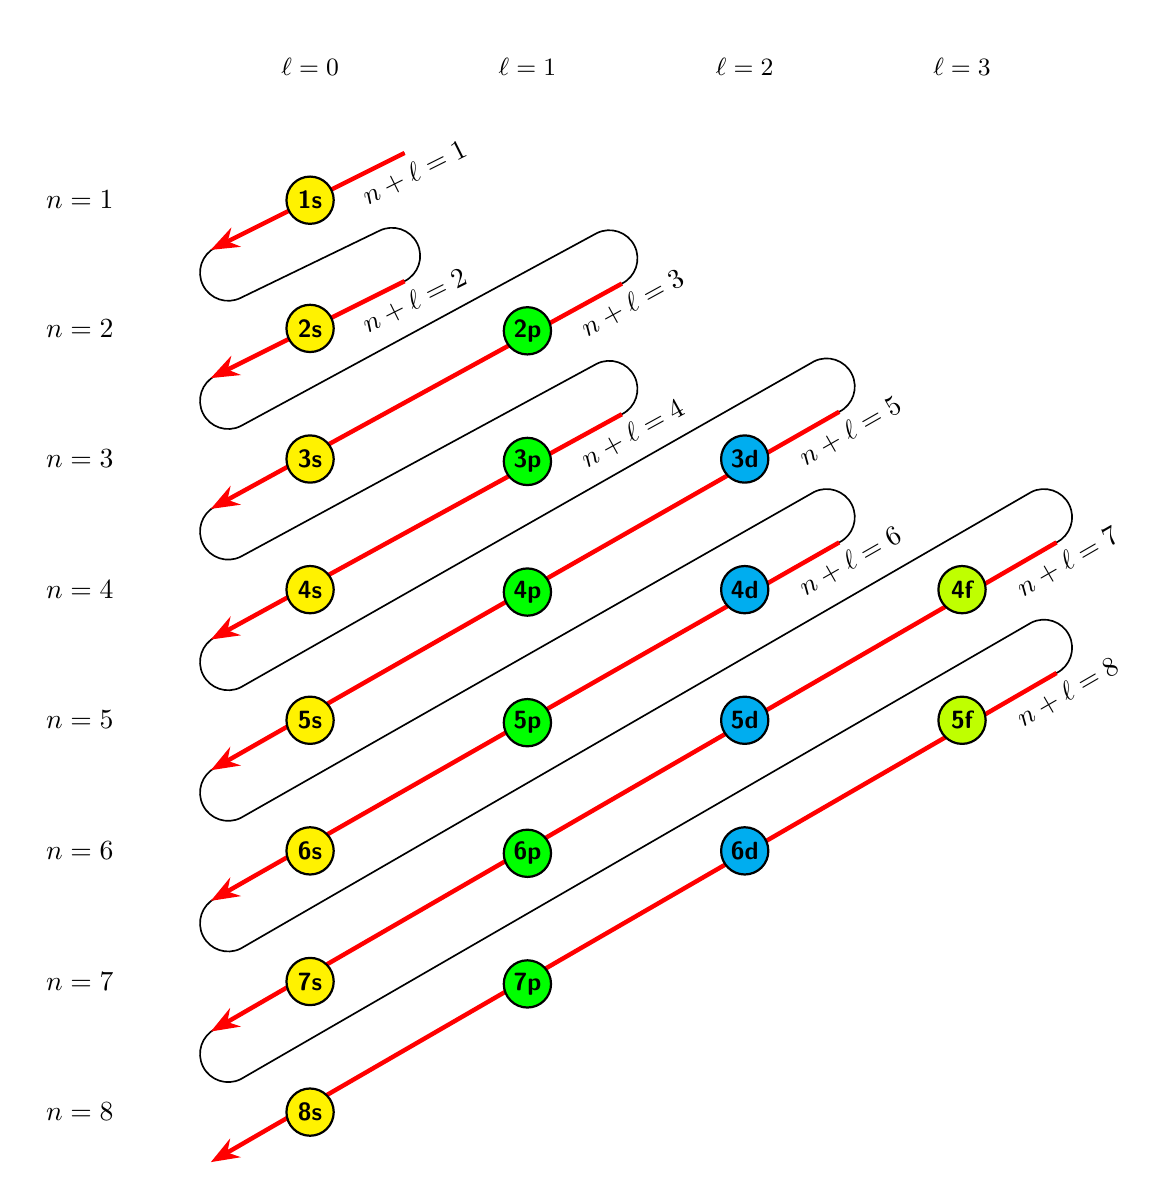
\begin{tikzpicture}[>=Stealth,line cap=round,line join=round]
\matrix (m) [%
    matrix of nodes,%
    column 2/.append style={nodes={s}},
    column 3/.append style={nodes={p}},
    column 4/.append style={nodes={d}},
    column 5/.append style={nodes={f}},
    row 1/.style={nodes={draw=none,fill=none}},%
    column1/.style={nodes={}},%
    row sep=\rowsep cm,%
    column sep=\colsep cm%
    ]%
{
          & $\ell=0$ & $\ell=1$ & $\ell=2$ & $\ell=3$ \\
    $n=1$ & 1s & & & \\
    $n=2$ & 2s & 2p & & \\
    $n=3$ & 3s & 3p & 3d & \\
    $n=4$ & 4s & 4p & 4d & 4f \\
    $n=5$ & 5s & 5p & 5d & 5f \\
    $n=6$ & 6s & 6p & 6d & \\
    $n=7$ & 7s & 7p & & \\
    $n=8$ & 8s & & & \\
};
\foreach \i in {2,3,...,9}{
        \path (m-\i-2) ++(-\deltax,-\deltay) coordinate (m-\i-2-L);
        \path (m-\i-2) ++(\deltax,\deltay) coordinate (m-\i-2-R);
        % \draw[red,ultra thick] (m-\i-2-L) -- (m-\i-2-R);
}
\foreach \x/\y in {3/3,4/3,4/3,4/4,5/4,5/5,6/5}{
    \path (m-\x-\y) ++(-\deltax,-\deltay) coordinate (m-\x-\y-L);
    \path (m-\x-\y) ++(\deltax,\deltay) coordinate (m-\x-\y-R);
    %  \draw[red,ultra thick] (m-\x-\y-L) -- (m-\x-\y-R);
}
\foreach \x/\y[count=\i] in {3/2,3/3,4/3,4/4,5/4,5/5,6/5}{
    \path (m-\x-\y-R) ++(\angleA:2*\myR) coordinate (tmp-\i);
}
\begin{scope}[on background layer]
\draw[semithick] 
(m-2-2-R) 
foreach \x/\y[count=\i] in {2/2,3/2,4/2,5/2,6/2,7/2,8/2}{
    -- (m-\x-\y-L)
    arc [start angle=\angleA,end angle=\angleB,radius=\myR]
    -- (tmp-\i)
    arc [start angle=\angleA,end angle=\angleC,radius=\myR]
}
-- (m-9-2-L)
;
\foreach \x/\y[%
    count = \i,%
    count = \j from 2%
] in {2/2,3/2,3/3,4/3,4/4,5/4,5/5,6/5}{
    \path[red,ultra thick] 
    (m-\x-\y-R) edge[->,shorten >=-2pt] node[at start,below,text=black,sloped] {$n+\ell=\i$} (m-\j-2-L);
}
\end{scope}
\end{tikzpicture}
\end{document}